%%% Mindmap of Information Theoretical Proof systems, useful for ZKP paradigms
%%% Luis Brandao: initial latex code 2020-Dec--2022-April
%%% Revised with Daniel Benarroch and Eran Tromer
%%% Keywords suggested by Yuval Ishai (2020-Dec)
%%% License: ZKProof @ CC-BY 4.0 --- Creative Commons Attribution 4.0 International

%%% Update LB 2022-July: hyperlinks added (will override the tooltips), line numbers added (incomplete code to control horizontal spacing per node)

\begingroup

%%% Definitions used for legend and tooltips

\def\extILC{Ideal Linear Commitment}
\def\extIOP{Interactive Oracle Proof}
\def\extIP{Interactive Proof}

\def\extIT{Information Theoretic}

\def\extQAP{Quadratic Arithmetic Program}
\def\extQSP{Quadratic Span Program}
\def\extSSP{Square Span Program}
\def\extPCP{Probabilistic Checkable Proof}
\def\extMPC{[Secure] Multi-Party Computation}
\def\extVOLE{Vector Oblivious Linear Evaluation}
\def\extZKP{Zero-Knowledge Proof}


%%% Styles for various levels os nodes
\newcommand{\styA}[1]{\scalebox{4}{\textbf{\subtab{#1}}}}
\newcommand{\styB}[1]{\scalebox{2.75}{\textbf{\subtab{#1}}}}
\newcommand{\styC}[1]{\scalebox{2}{\textbf{\subtab{#1}}}}
\newcommand{\styD}[1]{\scalebox{1.5}{\textbf{\subtab{#1}}}}


%\renewcommand{\pdftooltip}[2]{#1}

\let\hyperrefA\hyperref
\newcommand{\hyperrefB}[2][]{#2}


%%% Central node
\def\ZKP{\pdftooltip{ZKP}{Zero-Knowledge Proof}}
\def\ITproofs{\styA{\rule{0em}{1.5em}\hyperrefA[paradigms:IT]{\subtab{\pdftooltip{IT}{\extIT} Proof\\Systems}}\\for \ZKP{}s}}


%%% 1st order nodes
\def\ILC{\styB{\pdftooltip{\hyperrefA[paradigms:IT:ILC]{ILC}}{Ideal Linear Commitment}}}
\def\IOP{\styB{\pdftooltip{\hyperrefA[paradigms:IT:IOP]{IOP}}{\extIOP}}}
\def\LIOP{\styB{\pdftooltip{\hyperrefA[paradigms:IT:linear-IOP]{\subtab{Linear\\IOP}}}{Linear \extIOP}}}
\def\PCP{\styB{\pdftooltip{\hyperrefA[paradigms:IT:PCP]{PCP}}{\extPCP}}}
\def\LPCP{\styB{\pdftooltip{\hyperrefA[paradigms:IT:linear-PCP]{\subtab{Linear\\PCP}}}{Linear \extPCP}}}
\def\MiTH{\styB{\pdftooltip{\hyperrefA[paradigms:IT:MPC-in-the-head]{\subtab{MPC in\\the head}}}{[Secure] Multi-Party Computation in the Head}}}


%%% 2nd order nodes
\def\IPbased{\styC{\pdftooltip{\hyperrefA[paradigms:IT:linear-IOP:IP-based]{IP based}}{\extIP\ based}}}
\def\PolyIOP{\styC{\pdftooltip{\hyperrefA[paradigms:IT:linear-IOP:polynomial-IOP]{\subtab{Polynomial\\IOP}}}{Polynomial \extIOP}}}
\def\FLIOP{\styC{\pdftooltip{\hyperrefA[paradigms:IT:linear-IOP:fully-linear-IOP]{\subtab{Fully Linear\\IOP}}}{Fully-linear \extIOP}}}

\def\HadBased{\styC{\hyperrefA[paradigms:IT:linear-PCP:hadamard]{\subtab{Hadamard\\based}}}}
\def\LinePoint{\styC{\hyperrefA[paradigms:IT:linear-PCP:line-point]{\subtab{Line-Point}}}}
\def\FLPCP{\styC{\pdftooltip{\hyperrefA[paradigms:IT:linear-PCP:fully-linear]{\subtab{Fully Linear\\PCP}}}{Fully-linear \extPCP}}}
\def\QAP{\pdftooltip{QAP}{\extQAP}}
\def\QSP{\pdftooltip{QSP}{\extQSP}}
\def\SSP{\pdftooltip{SSP}{\extSSP}}
\def\FromQAPQSPSSP{\styC{\hyperrefA[paradigms:IT:linear-PCP:from-QAP]{\subtab{From \QAP/\\\QSP/\SSP}}}}

\def\ClassThreeCol{\styC{\hyperrefA[paradigms:IT:PCP:3-col]{\subtab{Classical\\3-coloring\\proof}}}}
\def\FromPCPTheo{\styC{\pdftooltip{\hyperrefA[paradigms:IT:PCP:from-PCP-theorem]{\subtab{From PCP\\theorem}}}{From \extPCP\ theorem}}}

\def\InterPCP{\styC{\pdftooltip{\hyperrefA[paradigms:IT:IOP:interactive-PCP]{\subtab{Interactive\\PCP}}}{Interactive \extPCP}}}
\def\FRI{\styC{\pdftooltip{\hyperrefA[paradigms:IT:IOP:fast-RS-IOPP]{\subtab{Fast RS\\IOPP}}}{Fast Reed-Solomon \extIOP\ of Proximity}}}



\newcounter{mylinenumberbeforefigure}
\setcounter{mylinenumberbeforefigure}{\value{linenumber}}
\addtocounter{mylinenumberbeforefigure}{-1}
\newcounter{cntNumLinesInFig}\setcounter{cntNumLinesInFig}{0}
\let\origthelinenumber\thelinenumber
% \setlinenumbermargin{#1}
% \renewcommand{\thelinenumber}{\hspace*{#1}\origthelinenumber}
% \renewcommand{\thelinenumber}{\makebox[0pt][l]{\value{linunumber}\hspace{#1}}}
\newlength{\myLNhorizoffset}
\setlength{\myLNhorizoffset}{-1.5em}

%%%%%%%%%%%%%%%%%%%%%%%%%%%%%%%%%%%%%%%%
\nolinenumbers
% LNO: line number ordering --- function that will (manually) inform the line number of each node
\newcommand{\LNO}[2][0pt]{\stepcounter{cntNumLinesInFig}
    \setcounter{linenumber}{\value{mylinenumberbeforefigure}}
		\addtocounter{linenumber}{#2}
    \setlength{\myLNhorizoffset}{#1}}
\begin{figure}[H]\centering  % !htb
\def\tmpfigcap{Various IT proof systems}
\refstepcounter{figure}\label{fig:it-mindmap}%
\hypertarget{ht:figure:\thefigure}{}
\addcontentsline{lof}{figure}{Figure~\thefigure{}: \tmpfigcap}
\nolinenumbers
\bookmarksetup{level=3,color=\colorbkmfig}
\bookmark[dest=ht:figure:\thefigure]{Figure~\thefigure}%

\begingroup  %% begin scope for changed \thelinenumbers
\let\tempthelinenumber\thelinenumber
\nolinenumbers


%\conditionalinternallinenumbers
%https://tex.stackexchange.com/questions/281226/tikz-getting-angles-in-mindmaps-right
\tikzset{grow cyclic list/.code={%
  \def\tikzgrowthpositions{{#1}}%
  \foreach \n [count=\i,remember=\i]in {#1}{}%
  \let\tikzgrowthpositionscount=\i%
  \tikzset{growth function=\tikzgrowcycliclist}}}
\def\tikzgrowcycliclist{%
  \pgftransformshift{%
    \pgfpointpolar{\tikzgrowthpositions[mod(\the\tikznumberofcurrentchild-1,\tikzgrowthpositionscount)]}%
      {\the\tikzleveldistance}}}

\makeatletter\tikzset{concept/.style={circle,draw=\tikz@concept@color,every concept}}\makeatother%
\centering%


% https://tikz.dev/tikz-shapes#section-nodes-multi
\vspace{1em}
%%%\centerline{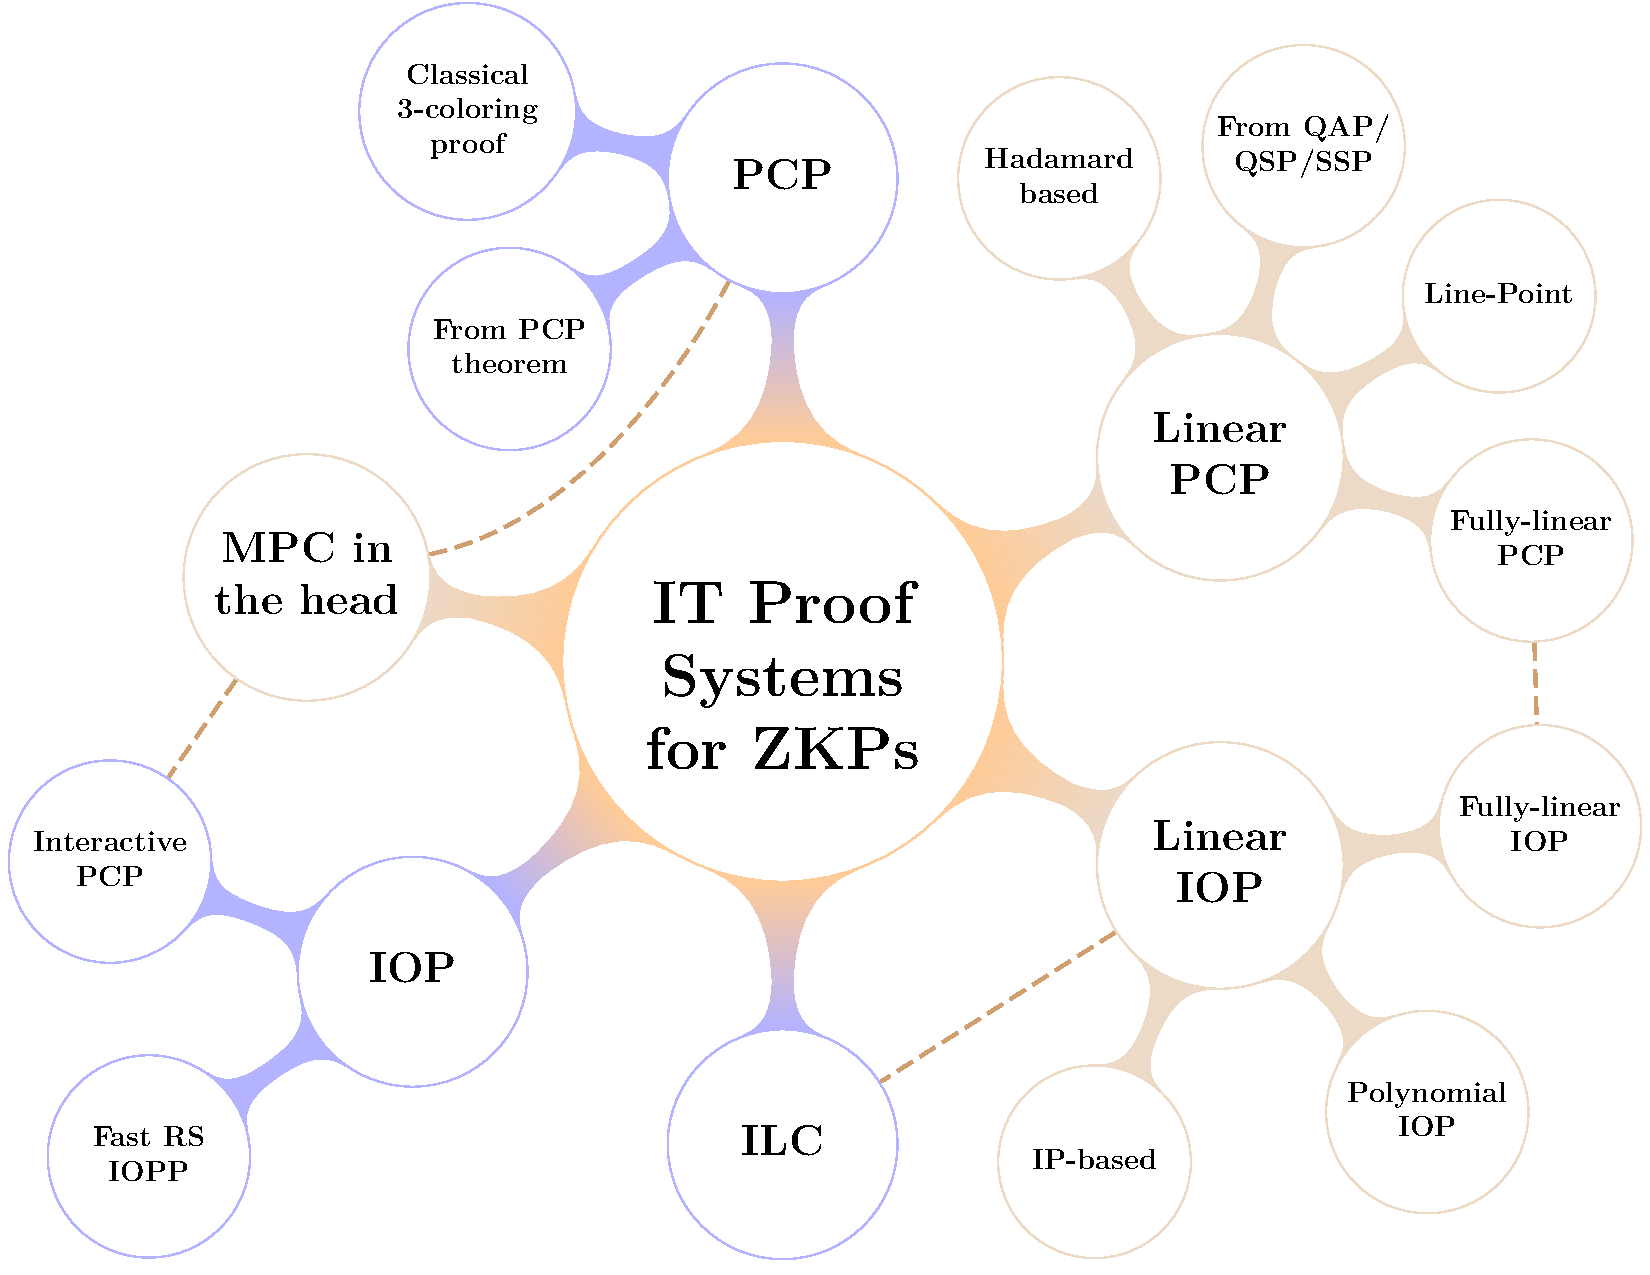
\includegraphics[width=.9\textwidth]{figs/mindmap-IT-proof-systems.pdf}} %width tailored to fit subsequent paragraph
\resizebox{.95\textwidth}{!}{\begin{tikzpicture}[rotate=+90,
execute at begin node = {\conditionalinternallinenumbers\renewcommand{\thelinenumber}{\scalebox{3}{\makebox[0pt][l]{\hspace*{\myLNhorizoffset}\tempthelinenumber}}}}
]     %%% if including legend and having margins .5in
\path[mindmap, grow cyclic, text width=4.4in, every node/.style=concept, align=flush center, concept color=orange!40, fill={none},
			%/.append style
			level 1/.style={text width=2.75in, level distance=6in, sibling angle=90, fill={none}},  
			level 2/.style={text width=2.33in, level distance=4.0in, sibling angle=45, fill={none}},
			level 3/.style={text width=1.15in, level distance=2.75in, sibling angle=45, fill={none}},
			%https://tex.stackexchange.com/questions/145991/inserting-special-border-to-tikz-mindmap
			marca/.append style={fill={none}}, outer sep=1pt
			]

%\setlength{\myLNhorizoffset}{-2.5em}
%node[concept, append after command=\pgfextra{\setlength{\myLNhorizoffset}{-5em}}] {\LNO[4em]{10}\ITproofs} %% \LNO[-1em]{10}
node[concept] {\LNO[4em]{10}\ITproofs} %% \LNO[-1em]{10}
%%%%
child[grow=0, concept color=blue!30] { node (pcp) {\LNO{3}\PCP} %%% \setlength{\myLNhorizoffset}{-1.5em}
	child[grow=78] { node {\LNO{1}\ClassThreeCol}}
	child[grow=122] { node {\LNO{6}\FromPCPTheo}}  %\zk-\PCP\\
}
child[grow=80, concept color=brown!30] { node (mpchead) {\LNO{9}\MiTH}
}
child[grow=130, concept color=blue!30] { node (iop) {\LNO{14}\IOP}
	child[grow=70] { node (interactivepcp) {\LNO{12}\InterPCP}}
	child[grow=125] { node {\LNO{17}\FRI}}
}
child[grow=180, concept color=blue!30] { node (ilc) {\LNO{16}\ILC}
}
child[grow=245, concept color=brown!30] { node (lineariop) {\LNO{13}\LIOP}    %color=teal!30
	child[grow=277] { node (FLIOP) {\LNO{11}\FLIOP}}
	child[grow=220.5] { node {\LNO{15}\PolyIOP}}
	child[grow=157] { node {\LNO{18}\IPbased}}
}
child[grow=-65, marca, concept color=brown!30] { node {\LNO{7}\LPCP} 
	child[grow=30] { node {\LNO{4}\HadBased}}
	child[grow=-15] { node {\LNO{2}\FromQAPQSPSSP}}
	child[grow=-60] { node {\LNO{5}\LinePoint}}
	child[grow=-105] { node (FLPCP) {\LNO{8}\FLPCP}}
};


%%% https://tex.stackexchange.com/questions/266983/adding-an-independent-small-node-in-a-mind-map
\begin{pgfonlayer}{background}
    %\draw [left color=blue, right color=green!50!black, draw=white, decorate,decoration=circle connection bar] (mpchead) -- (pcp);
	\draw[dash pattern=on 16pt off 8pt,line width=3pt, brown!75] (mpchead) to[out=-50,in=180] (pcp);
    \draw[dash pattern=on 16pt off 8pt,line width=3pt, brown!75] (mpchead) -- (interactivepcp);
    \draw[dash pattern=on 16pt off 8pt,line width=3pt, brown!75] (FLPCP) -- (FLIOP);
	\draw[dash pattern=on 16pt off 8pt,line width=3pt, brown!75] (lineariop) -- (ilc);  %to[out=160,in=-20]

\end{pgfonlayer}

\end{tikzpicture}
} %% end of \restoline

\endgroup  %% end scope for changed \thelinenumbers

\addtocounter{mylinenumberbeforefigure}{\value{cntNumLinesInFig}}
\setcounter{linenumber}{\value{mylinenumberbeforefigure}}
\stepcounter{linenumber}

\vskip0pt
\vspace{1.5em}
\nolinenumbers
\restoline{\begin{minipage}[t]{1.07\textwidth}\setlinenumbermargin{.4em}{}\conditionalinternallinenumbers
\textbf{Legend:} 
\textbf{Fast RS IOPP} (aka FRI: Fast Reed-Solomon IOP of Proximity);
\textbf{ILC} (\extILC); 
\textbf{IOP} (\extIOP); 
\textbf{IP} (\extIP);
\textbf{IT} (\extIT);
\textbf{MPC} (\extMPC); 
\textbf{PCP} (\extPCP); 
\textbf{QAP} (\extQAP); 
\textbf{QSP} (\extQSP); 
\textbf{SSP} (\extSSP); 
\textbf{ZKP} (Zero-Knowledge Proof).
\end{minipage}}

\conditionalinternallinenumbers % to get line number in caption of figure
\vskip.75em\textbf{Figure \thefigure. }\tmpfigcap
%%% \caption{\label{fig:it-mindmap}}
\end{figure}

\endgroup


\linenumbers
